\documentclass[11pt, a4paper]{article}
\usepackage[utf8]{inputenc}
\usepackage{graphicx}
\usepackage[left=2.5cm, right=2.5cm, top=2.5cm, bottom=2.5cm]{geometry}
\usepackage{hyperref}
\usepackage{fancyhdr}
\usepackage{tabularx} 
\usepackage{float}
\usepackage[style=apa, backend=biber, sortcites=true, sorting=nyt, doi=true, url=true, isbn=false, eprint=false]{biblatex}
\DeclareLanguageMapping{american}{american-apa} 
\addbibresource{references.bib}
\usepackage[table,xcdraw]{xcolor}
% Custom header/footer for page numbering
\pagestyle{fancy}
\fancyhf{}
\rhead{Page \thepage}
\lhead{}
\cfoot{}



% Title Page
\title{Patterns Linking Health Expenditure, Health Outcomes, and GDP: A Principal Component Analysis}
\author{Agata Zabuska}
\date{}
\begin{document}

% The following command creates the title page
\maketitle
\thispagestyle{empty} % No page number on the title page

% Table of Contents
\newpage
\tableofcontents
\thispagestyle{empty} % No page number on the table of contents
\newpage

% Abstract
\section*{Abstract}
\addcontentsline{toc}{section}{Abstract}
\begin{center}
    \textbf{Abstract}
\end{center}
\vspace{1em}
This study examines the multivariate relationship between healthcare expenditure, GDP per capita, and health outcomes on a global scale. Using exploratory data analysis (EDA), correlation analysis, and Principal Component Analysis (PCA), we consistently found a strong, statistically significant positive correlation between a nation's GDP per capita and its healthcare investment and health outcomes. High GDP per capita was strongly associated with increased healthcare spending and improved metrics, such as life expectancy and the availability of medical professionals.

A key contribution of this research is the development of a composite index using PCA. This index provides a unified metric for benchmarking and evaluating the overall performance of national health systems. Analysis of this index revealed a significant disparity in health system performance across countries, with high-income nations like the United States, Norway, and Switzerland ranking as top performers, while lower-income nations such as Burkina Faso, Mozambique, and Lao PDR occupy the lower end of the spectrum. These findings underscore the link between economic prosperity and healthcare system strength and effectiveness.

---

% Introduction
\section{Introduction}

Healthcare expenditure constitutes a significant share of national budgets across both developed \parencite{Sterlin2024} and developing economies \parencite{health}. It represents the allocation of financial and material resources to restore, maintain, and improve population health. The origins of modern national healthcare schemes can be traced back to the reforms of German Chancellor Otto von Bismarck in the late nineteenth century \parencite{busse2017}. Amid growing political unrest fueled by European labor movements, establishing comprehensive health coverage was seen as a way to alleviate discontent among German workers. This pioneering system, funded jointly by workers and employers, provided sick leave and medical care for blue-collar workers.  

Empirical evidence suggests that the introduction of statutory health insurance in Germany contributed not only to substantial improvements in life expectancy \parencite{bauernschuster2020} but also coincided with GDP growth \parencite{article} during the late nineteenth and early twentieth centuries. This historical example underscores the potential link between health and economic development: healthier populations tend to be more productive, while economic growth enables governments to invest in public health systems, thereby further improving life expectancy.  

Testing whether such a relationship exists in contemporary settings requires accounting for the complexity of modern healthcare financing. Unlike the original Bismarck system, current healthcare schemes operate through a diverse array of funding channels, including public insurance funded through taxation, private health insurance, out-of-pocket payments, and international aid in some low-income countries. These financing mechanisms interact with one another, making it essential to employ statistical techniques capable of capturing complex, multidimensional relationships across countries.  

To address this issue and test the hypothesis that a link exists between healthcare expenditure, health outcomes, and GDP, this study employs Principal Component Analysis (PCA), a widely used multivariate technique that reduces data dimensionality while preserving as much variance as possible \parencite{Jolliffe2002}. PCA enables the construction of composite indices that capture the underlying structure of healthcare expenditure and outcome variables, thereby facilitating cross-country comparisons and the identification of key contributing factors.   
---

% Materials and Methods
\section{Materials and Methods}
\label{sec:materials_methods}

The data used in this study was obtained from the World Bank Group's Health Nutrition and Population Statistics and World Development databases, available at https://databank.worldbank.org/ (accessed on September 19, 2025). The Health Nutrition and Population Statistics database contains diverse information on health expenditure and health systems across countries. Feature selection was guided by the World Health Organization's handbook on health system indicators, which outlines key variables for evaluating health systems \parencite{WHO2010}. GDP per capita values per country were obtained from the World Development database. Both datasets were merged using the country code to create a unified dataset. Table 1 lists all features included in the final dataset along with their descriptions.

% Please add the following required packages to your document preamble:
% \usepackage[table,xcdraw]{xcolor}
% Beamer presentation requires \usepackage{colortbl} instead of \usepackage[table,xcdraw]{xcolor}
\begin{table}[ht]
\begin{tabularx}{\textwidth}{lXl l}
\rowcolor[HTML]{000000} 
{\color[HTML]{FFFFFF} Feature} & {\color[HTML]{FFFFFF} Description} & {\color[HTML]{FFFFFF} Unit} & {\color[HTML]{FFFFFF} Type} \\
Country Name & Name of the country & - & character \\
HealthExp(\% of GDP) & Current health expenditure (\% of GDP) & \% & numeric \\
HealthExp(current US\$) & Current health expenditure per capita & \$ & numeric \\
DomesticExp(\% of HE) & Domestic general government health expenditure (\% of current health expenditure) & \% & numeric \\
DomesticExp(\% of GDP) & Domestic general government health expenditure (\% of GDP) & \% & numeric \\
DomesticExp(current US\$) & Domestic general government health expenditure per capita (current US\$) & \$ & numeric \\
PrivExp(current US\$) & Domestic private health expenditure per capita (current US\$) & \$ & numeric \\
PrivExp(\% of HE) & Domestic private health expenditure (\% of current health expenditure) & \% & numeric \\
ExternalExp(current US\$) & External health expenditure per capita (current US\$) & \$ & numeric \\
Out-of-pocketExp(\% of HE) & Out-of-pocket expenditure (\% of current health expenditure) & \% & numeric \\
Out-of-pocketExp(current US\$) & Out-of-pocket expenditure per capita (current US\$) & \$ & numeric \\
Physicians & Physicians (per 1,000 people) & - & numeric \\
Hospital beds & Hospital beds (per 1,000 people) & - & numeric \\
Nurses and midwives & Nurses and midwives (per 1,000 people) & - & numeric \\
Life expectancy at birth & Life expectancy at birth, total (years) & - & numeric \\
Mortality rate, infant & Mortality rate, infant (per 1,000 live births) & - & numeric \\
Maternal mortality ratio & Maternal mortality ratio (modeled estimate, per 100,000 live births) & - & numeric \\
Mortality rate, under-5 & Mortality rate, under-5 (per 1,000) & - & numeric \\
GDP per capita & GDP per capita (current US\$) & \$ & numeric
\end{tabularx}
\end{table}

After merging, each country had a combination of health and economic variables. Data cleaning steps included eliminating records with missing values. The workflow consisted of the following steps:

\begin{enumerate}
\item Data collection: Relevant databases were identified, and variables were selected based on literature and the study objectives.
\item Dataset creation: Health and economic datasets were merged using country codes to create a unified structure.
\item Data pre-processing: Records with empty values were identified and deleted. Filling in empty values was not possible due to non-random distribution of elements. 
\item Exploratory data analysis (EDA): Pair plots were used to visualize relationships and data distributions.
\item Initial per country analysis: An initial country-level analysis was conducted using bar charts to highlight the top twenty countries with the highest values for key indicators, including life expectancy, health expenditure per capita, and health expenditure as a percentage of GDP.
\item Data standardization: Numerical variables were standardized by subtracting the mean and dividing by the standard deviation, ensuring each feature had a mean of 0 and standard deviation of 1.
\item Correlation analysis: A correlation matrix using Pearson coefficients was computed to assess the strength and direction of relationships among variables.
\item Principal Component Analysis (PCA): PCA was conducted by computing the covariance matrix, extracting eigenvectors (principal component directions) and eigenvalues (variance explained), and projecting the standardized data onto the principal components.
\end{enumerate}

---

% Results and Discussion
\section{Results and Discussion}
\label{sec:results_discussion}

An initial analysis was conducted by plotting countries with the highest values for Life expectancy, Current health expenditure (\% of GDP), Current health expenditure per capita. As shown in Figure \ref{fig:P1}, life expectancy among the top twenty countries is relatively close, oscillating around 80 years. In contrast, Figure \ref{fig:P2} and Figure \ref{fig:P3} illustrate the large disparity in health expenditure values among the top twenty countries, with the United States ranked first in both categories.

\begin{figure}[H]
\centering
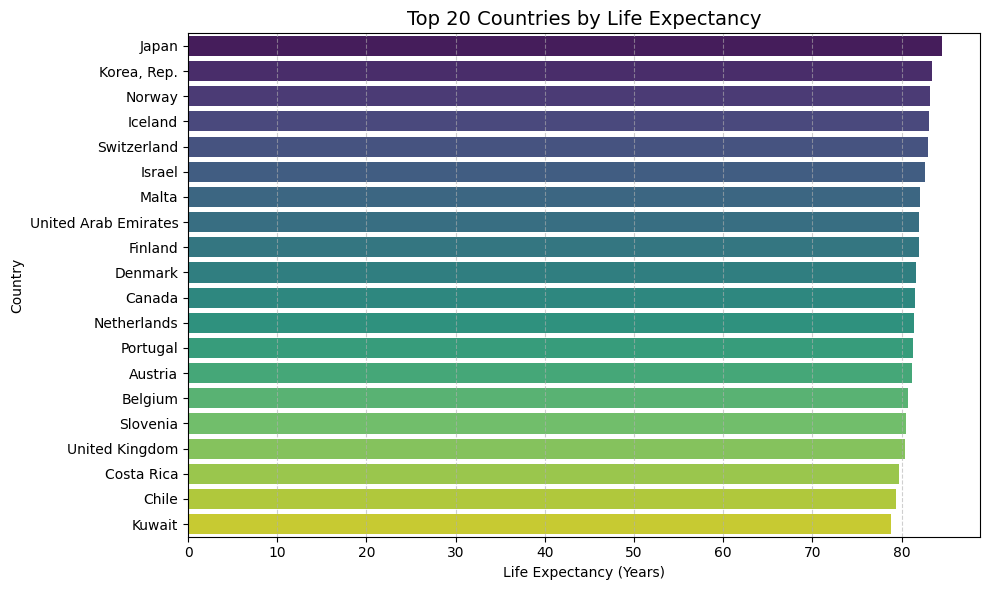
\includegraphics[width=0.5\linewidth]{output_1.png}
\caption{Bar chart showing twenty countries with highest life expectancy.}
\label{fig:P1}
\end{figure}

\begin{figure}[H]
\centering
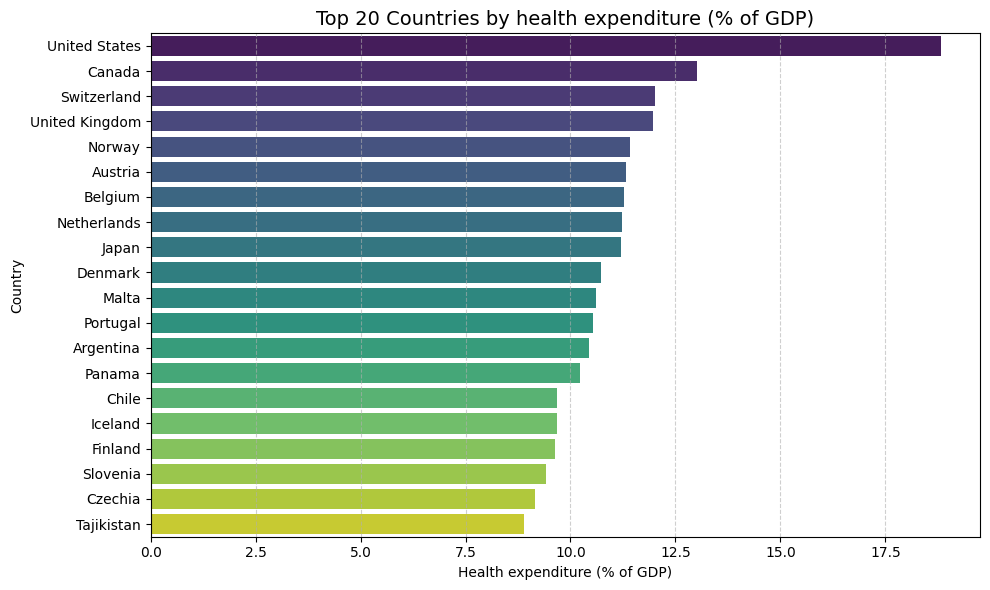
\includegraphics[width=0.5\linewidth]{output_2.png}
\caption{Bar chart showing twenty countries with highest health expenditure as percentage of GDP.}
\label{fig:P2}
\end{figure}

\begin{figure}[H]
\centering
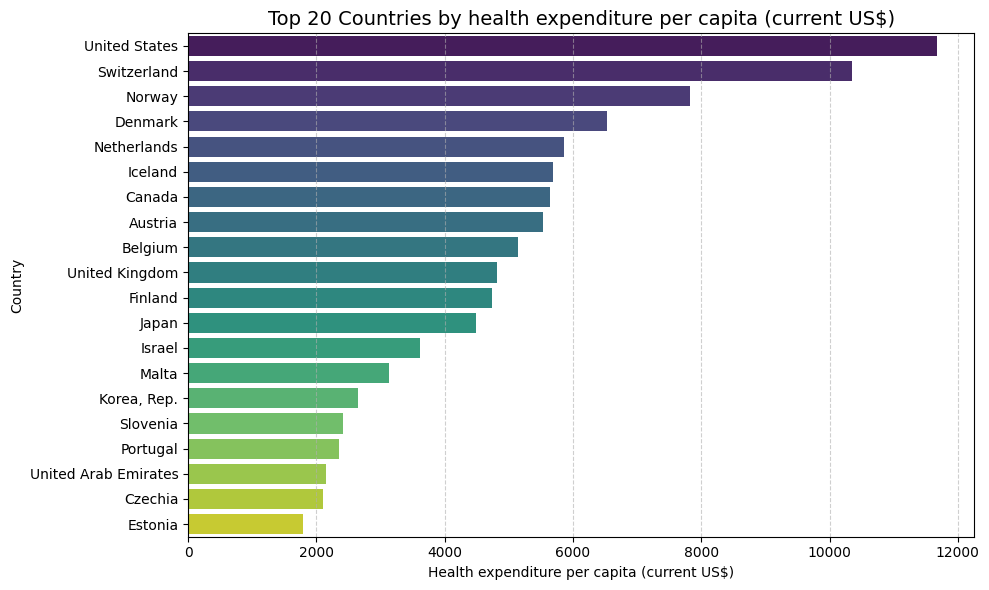
\includegraphics[width=0.5\linewidth]{output_3.png}
\caption{Bar chart showing twenty countries with highest health expenditure per capita.}
\label{fig:P3}
\end{figure}


Exploratory Data Analysis (EDA) was conducted to examine correlations, trends, and potential outliers in the dataset prior to applying dimensionality reduction techniques. The main objective was to understand the relationships between health expenditure, economic indicators, and health outcomes.

For this part only the numeric features were taken into consideration. The pairwise relationships between variables were visualized using a pair plot (Figure \ref{fig:1}). This visualization revealed a strong positive correlation between GDP per capita and most health expenditure variables, including Current health expenditure (\% of GDP), 
Current health expenditure per capita, Domestic general government health expenditure (\% of current health expenditure), Domestic general government health expenditure (\% of GDP), and Out-of-pocket expenditure per capita (current US\$). Furthermore, other key healthcare indicators— Physicians (per 1,000 people), Nurses and midwives (per 1,000 people), and Life expectancy at birth, total (years)—also demonstrated a positive correlation with GDP per capita. In contrast, variables related to mortality rates did not exhibit a significant correlation with GDP.

\begin{figure}[H]
\centering
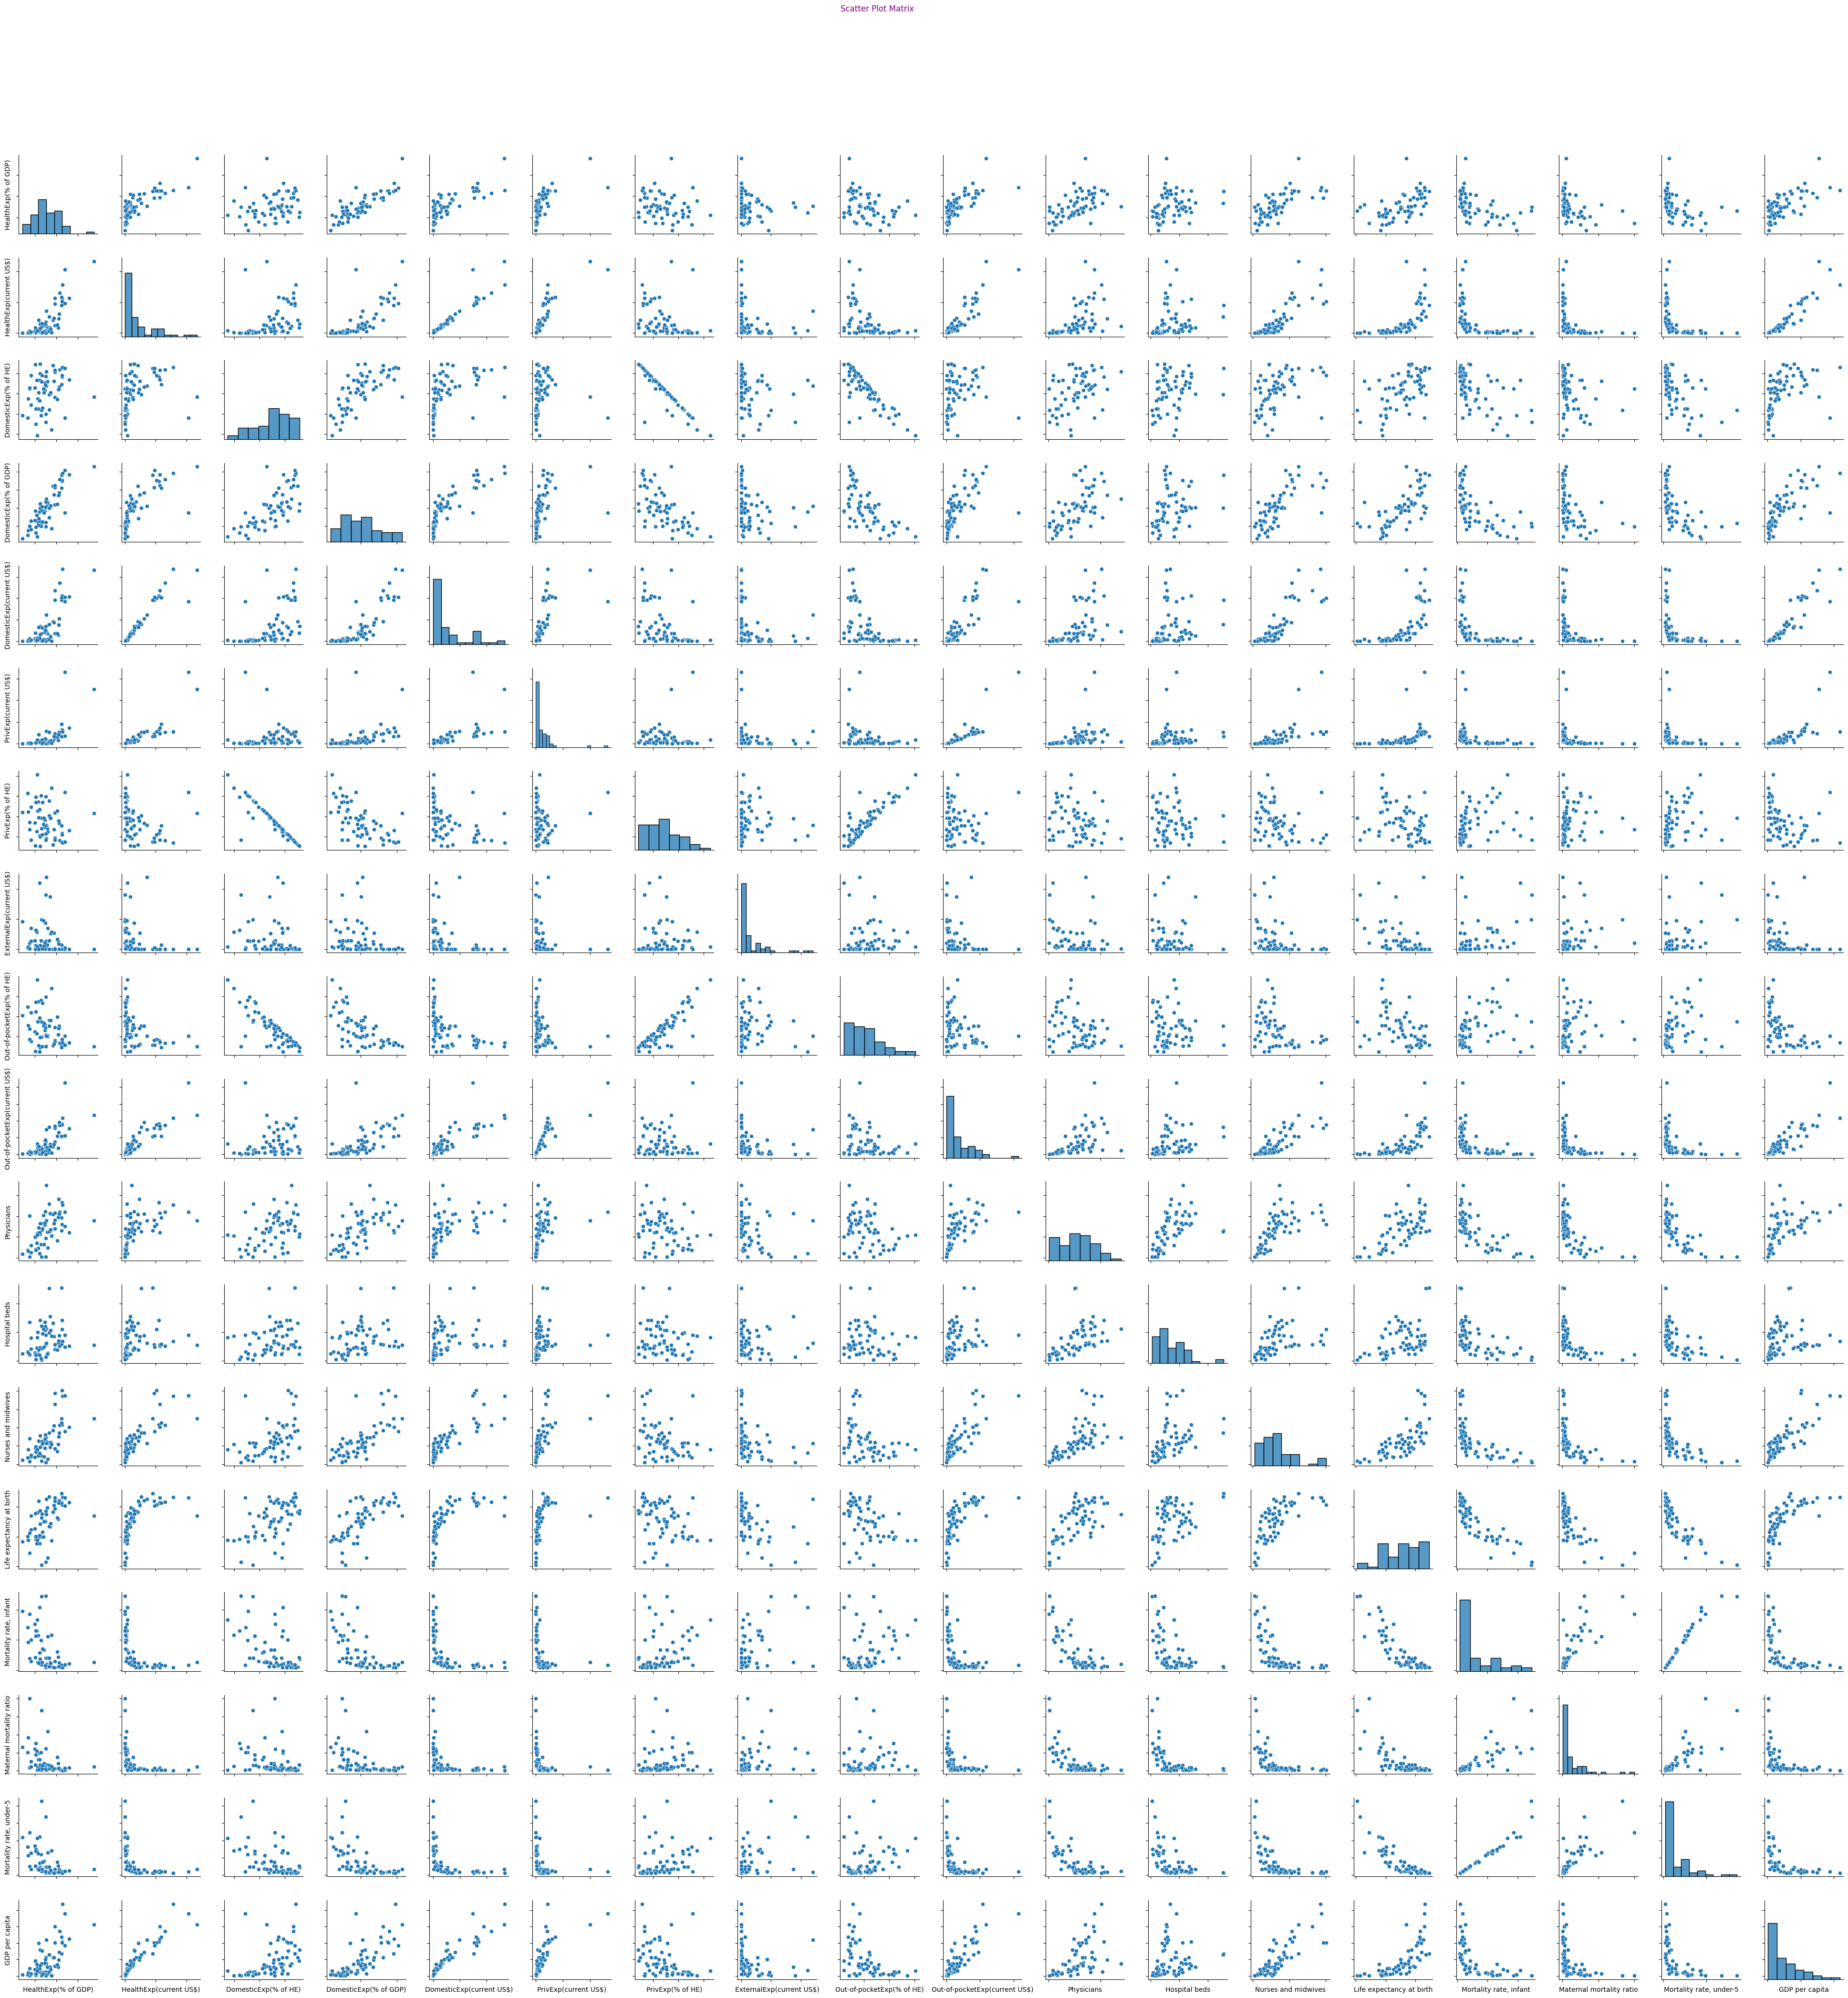
\includegraphics[width=0.5\linewidth]{output_14.png}
\caption{Pair plot illustrating pairwise relationships among variables.}
\label{fig:1}
\end{figure}

To further inspect these observations, a correlation matrix was computed using Pearson correlation coefficients (Figure \ref{fig:4}). The heatmap visualization highlights strong positive correlations among most health expenditure indicators and GDP per capita, confirming patterns observed in the earlier exploratory steps.

\begin{figure}[H]
\centering
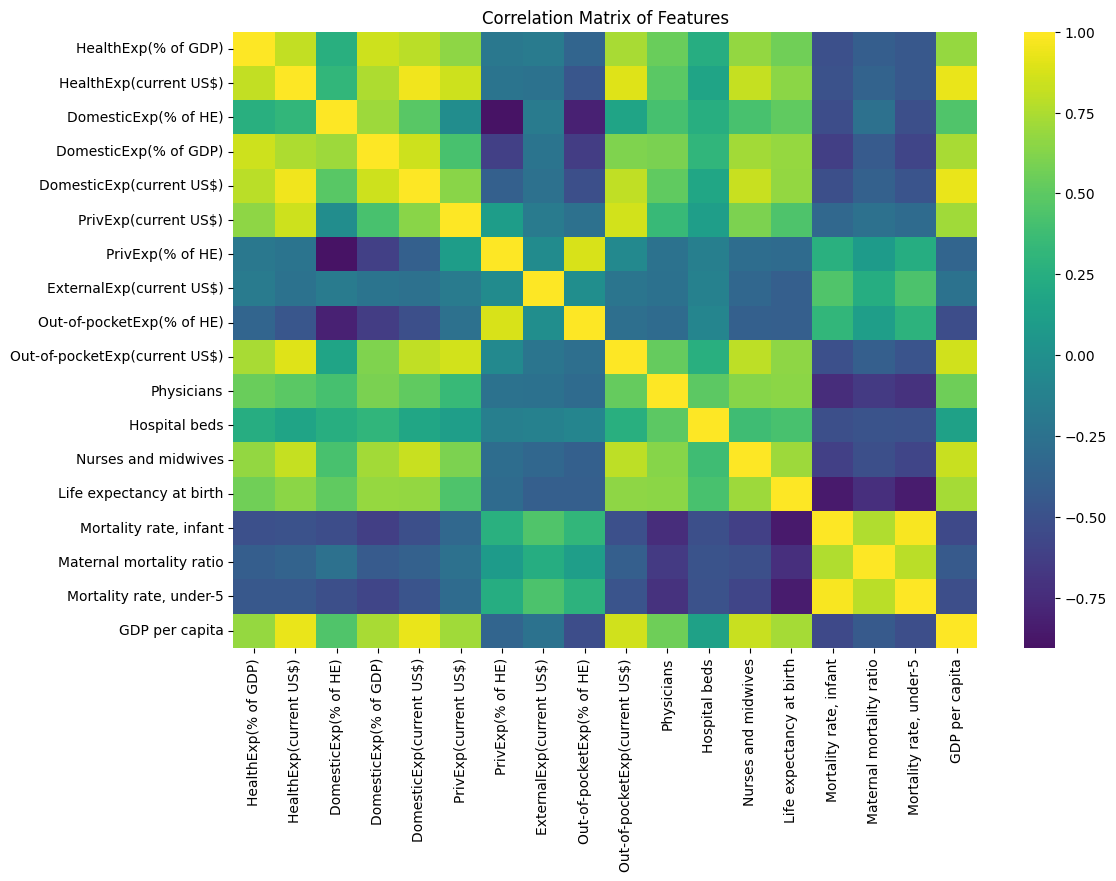
\includegraphics[width=0.5\linewidth]{output_17.png}
\caption{Correlation matrix illustrating the strength and direction of correlations among variables.}
\label{fig:4}
\end{figure}

Following the exploratory data analysis (EDA), Principal Component Analysis (PCA) was conducted, excluding the feature \textit{GDP} to ensure that principal components reflected only health expenditure and healthcare outcome variables. Figure \ref{fig:5} presents the scree plot, illustrating the variance explained by each component and guiding the selection of the optimal number of components. While the "elbow" criterion indicates that the first two components capture over 65\% of the variance, a cumulative variance threshold approach was adopted, targeting over 80\%. Under this criterion, the first four principal components were retained for further analysis, including variable contribution assessment. This analysis quantified the contribution of each variable to the principal components based on their correlations. As shown in Figure \ref{fig:7}, variables representing different healthcare expenditure channels, along with factors such as physicians (per 1,000 people), nurses and midwives (per 1,000 people), life expectancy at birth (years), and hospital beds (per 1,000 people), were the primary contributors to the variance explained by the first principal component.

\begin{figure}[H]
\centering
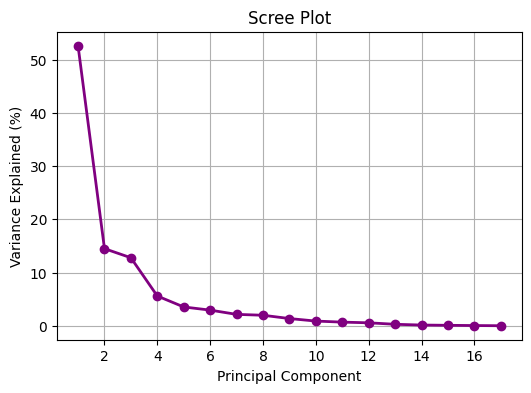
\includegraphics[width=0.5\linewidth]{output_6.png}
\caption{Percentage of variance explained by principal components.}
\label{fig:5}
\end{figure}

\begin{figure}[H]
\centering
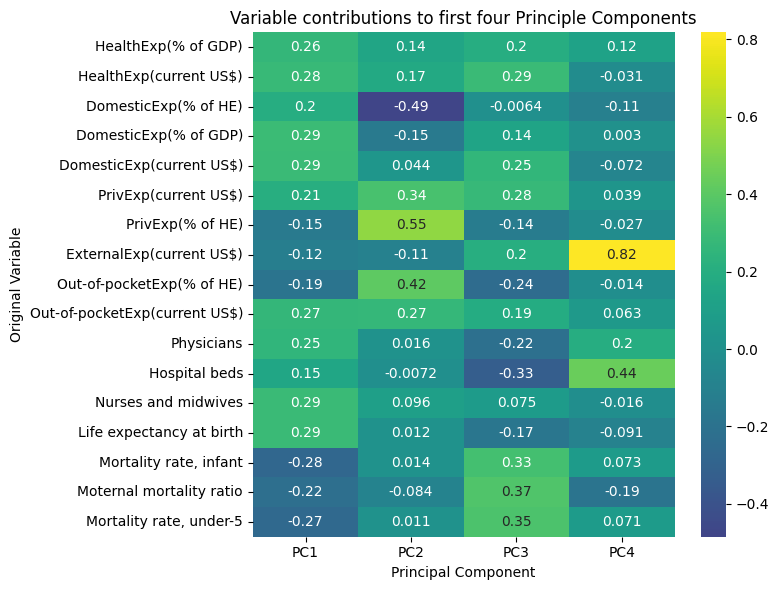
\includegraphics[width=0.5\linewidth]{output_10.png}
\caption{Variable contribution.}
\label{fig:7}
\end{figure}

To evaluate the initial hypothesis regarding the relationship between healthcare expenditure, healthcare outcomes, and GDP, a regression analysis was performed. Figure \ref{fig:6} indicates a positive correlation, showing that higher GDP per capita is associated with increased healthcare expenditure and improved healthcare outcomes.

\begin{figure}[H]
\centering
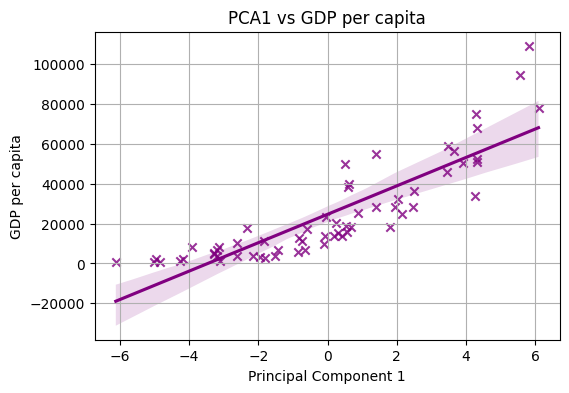
\includegraphics[width=0.5\linewidth]{output_7.png}
\caption{First principle component correlation with GDP}
\label{fig:6}
\end{figure}

PCA not only validated the initial findings but also provided a means to summarize healthcare expenditure and outcome variables into principal component scores, enabling each country to be assigned a single composite measure. For the first principal component, which captures the largest share of variance, Figure \ref{fig:8} highlights the highest- and lowest-performing countries. The results revealed that the United States, Norway, and Switzerland rank among the top performers, whereas Burkina Faso, Mozambique, and Lao PDR occupy the lower end of the spectrum.

\begin{figure}[H]
\centering
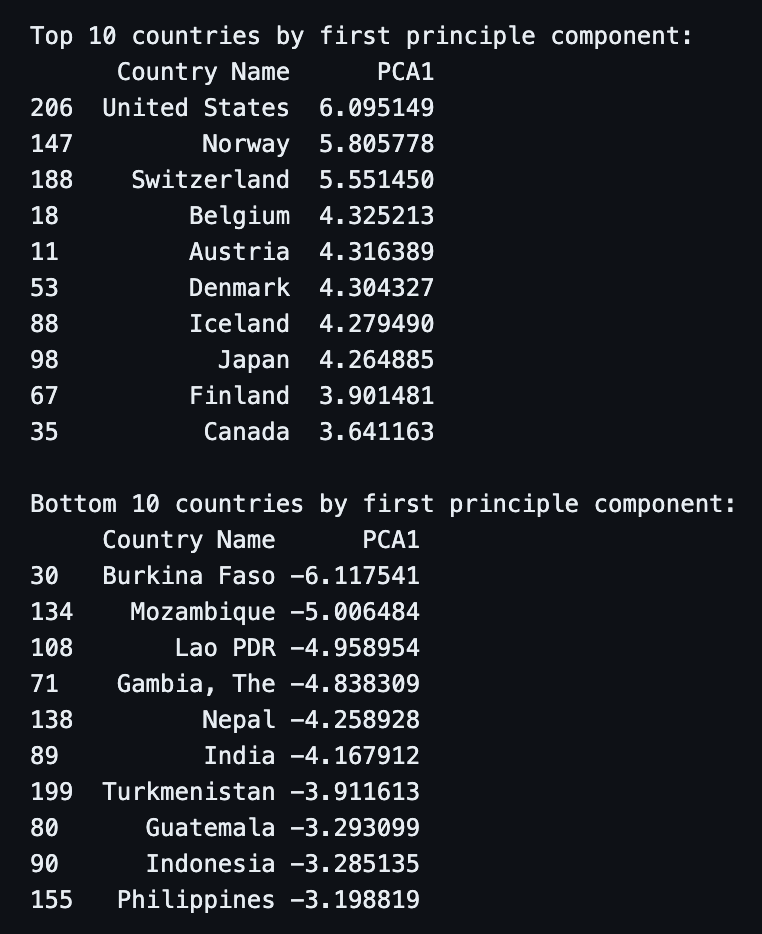
\includegraphics[width=0.5\linewidth]{scr6.png}
\caption{Countries ranked by first principle component values}
\label{fig:8}
\end{figure}
---

% Separate Results and Discussion (if you prefer)
% Alternatively, you can use two separate sections instead of the combined one.
% You can comment out the above section and uncomment the following two.
%\section{Results}
%\label{sec:results}
%Present your findings clearly, using figures, tables, and text to showcase your data.
%
%\section{Discussion}
%\label{sec:discussion}
%Discuss the meaning of your results. Explain what they tell us, their limitations, and their broader implications.

---

% Conclusions
\section{Conclusion}
\label{sec:conclusion}

This study examined the complex relationship between healthcare expenditure, health outcomes, and economic development by analyzing data from multiple countries. By employing Principal Component Analysis , we were able to address the multidimensional nature of modern healthcare financing and its diverse metrics.  

Exploratory data analysis and the subsequent correlation matrix revealed strong positive correlations among most health expenditure indicators and GDP per capita. This fundamental relationship was further supported by regression analysis on the first principal component, which effectively summarized multiple healthcare variables into a single composite score. This composite measure provided a unified metric for cross-country comparisons. Ranking countries by this score highlighted substantial disparities, with high-income nations such as the United States and Norway ranking at the top, while lower-income nations appeared at the bottom. These contrasts underscore the persistent global inequalities in health and economic outcomes.  

The strong positive correlation between economic prosperity and healthcare metrics suggests the existence of a general pattern: nations able to invest more in health tend to achieve better health outcomes, which in turn fosters a more productive workforce and further economic development. However, it is important to emphasize that the techniques deployed in this study identify patterns but cannot fully explain causality. PCA does not determine whether higher GDP leads to longer life expectancy or whether healthier populations drive economic growth. Future research could explore these relationships using causal inference frameworks.  

Additionally, PCA is inherently descriptive and relies solely on the variables included in the analysis. Omitted variables relevant to the underlying phenomena could impact the principal components' values. Consequently, the loadings and interpretations of the components may be biased, and the derived indices may not fully capture the real structure of healthcare expenditure and outcomes. It is important to remember that careful selection of variables, supported by experts with domain knowledge, is essential to mitigate this limitation. 


\printbibliography
\end{document}